% It is an example file showing how to use the 'sigkddExp.cls' 
% LaTeX2e document class file for submissions to sigkdd explorations.
% It is an example which *does* use the .bib file (from which the .bbl file
% is produced).
% REMEMBER HOWEVER: After having produced the .bbl file,
% and prior to final submission,
% you need to 'insert'  your .bbl file into your source .tex file so as to provide
% ONE 'self-contained' source file.
%
% Questions regarding SIGS should be sent to
% Adrienne Griscti ---> griscti@acm.org
%
% Questions/suggestions regarding the guidelines, .tex and .cls files, etc. to
% Gerald Murray ---> murray@acm.org
%

\documentclass{sigkddExp}

\begin{document}
%
% --- Author Metadata here ---
% -- Can be completely blank or contain 'commented' information like this...
%\conferenceinfo{WOODSTOCK}{'97 El Paso, Texas USA} % If you happen to know the conference location etc.
%\CopyrightYear{2001} % Allows a non-default  copyright year  to be 'entered' - IF NEED BE.
%\crdata{0-12345-67-8/90/01}  % Allows non-default copyright data to be 'entered' - IF NEED BE.
% --- End of author Metadata ---

\title{Covid-19 X-ray Image Classification}
%\subtitle{[Extended Abstract]
% You need the command \numberofauthors to handle the "boxing"
% and alignment of the authors under the title, and to add
% a section for authors number 4 through n.
%
% Up to the first three authors are aligned under the title;
% use the \alignauthor commands below to handle those names
% and affiliations. Add names, affiliations, addresses for
% additional authors as the argument to \additionalauthors;
% these will be set for you without further effort on your
% part as the last section in the body of your article BEFORE
% References or any Appendices.

\numberofauthors{4}
%
% You can go ahead and credit authors number 4+ here;
% their names will appear in a section called
% "Additional Authors" just before the Appendices
% (if there are any) or Bibliography (if there
% aren't)

% Put no more than the first THREE authors in the \author command
%%You are free to format the authors in alternate ways if you have more 
%%than three authors.

\author{
    %
    % The command \alignauthor (no curly braces needed) should
    % precede each author name, affiliation/snail-mail address and
    % e-mail address. Additionally, tag each line of
    % affiliation/address with \affaddr, and tag the
    %% e-mail address with \email.
    \alignauthor Maneesh Kumar Singh\\
    \affaddr{University of Illinois at Urbana-Champaign}\\
    \email{mksingh4@illinois.edu}
    \alignauthor Raman Walwyn-Venugopal\\
    \affaddr{University of Illinois at Urbana-Champaign}\\
    \email{rsw2@illinois.edu}
    \alignauthor Satish Reddy Asi\\
    \affaddr{University of Illinois at Urbana-Champaign}\\
    \email{sasi2@illinois.edu}
    \alignauthor Srikanth Bharadwaz Samudrala\\
    \affaddr{University of Illinois at Urbana-Champaign}\\
    \email{sbs7@illinois.edu}
}

\date{28 March 2021}
\maketitle
\begin{abstract}
    Objective
    Improve COVID-19 detection using X-Ray images by combining two recent approaches. FLANNEL (Focal Loss based Neural Network Ensembl
    Materials and Methods
    Use segmentation networks to create masks for the chest area. Feed random k-patches of masked area to base and ensemble models for FLANNEL.
    Results
    We are able to reproduce FLANNEL and base models results using the new datasets. We were also able to reproduce Patch-by-patch classification using X-ray images.
    Discussion
    We saw improvement in FLANNEL using the new dataset where COVID-19 images are more which were present when the FLANNEL paper was written.
    Conclusion
    We are integrating a segmentation network with FLANNEL and testing.
    Detecting COVID-19 using Chest X-Ray (CXR) images is becoming increasingly popular in deep learning research. When training deep neural networks, large and balanced datasets are preferred. However, since COVID-19 is new, the amount of CXR images available for it are limited which poses a challenge for training deep neural networks. Existing research has shown different approaches to address this imbalanced data issue. Two notable studies are FLANNEL[5]  an ensemble based network with focal loss and a patch-based classifier[4]  that works on segmented versions of the lung contours. We propose merging these two concepts together to improve performance of detecting COVID-19 in CXR images.

\end{abstract}

\section{Introduction}
COVID-19 pandemic has ravaged the world on an unprecedented scale. By April 2021, 141 million people have been infected and there have been 3.01 million deaths. X-ray imaging plays an important role in the diagnosis of COVID-19 and other pneumonia. It is often the first-line diagnosis in many cases. Using deep learning for X-ray classification is an ongoing research area and recently there have been promising models proposed for COVID-19 classification. The problem that all of these models face is an imbalance dataset due to the limited number of COVID CXR images available.

FLANNEL is a COVID-19 CXR classification model proposed by Zhi Qiao et al. [5]that has been shown to accurately detect COVID-19 even when trained with only 100 available COVID-19 x-ray images. There are core components for the FLANNEL architecture, the first is that it uses an ensemble[2] of five independent base learners that predict the classification of the CXR. Each of the predictions are then passed through another network to determine the final prediction classification. The goal of the ensemble is to increase the robustness and accuracy of the network since each base learner should capture patterns in the images independently. The second core component for the FLANNEL is its use of the special Focal Loss[3] function, a modification of the standard cross-entropy loss that places a focus on the imbalance negatives by applying down-weights to well-classified examples. Focal Loss has been known to improve performance for imbalanced datasets.

Park et. al[4] has also created a deep learning model that has been proven to be effective on detecting COVID-19 when trained with limited datasets. The approach taken was to first detect lung contours of the CXR and perform segmentation. The motivation for performing segmentation prior is so that the model focuses on classifying that area since it’s the primary region of interest used to perform analysis. This makes the model less susceptible to noise happening outside the lung region. After the lungs have been segmented, patch-based classification is performed. Patch-based classification involves selecting random crops or patches across the image a set number of times and then performing classification on each patch. Afterwards, the final prediction of the image is made by majority voting based on the prediction of each patch. From the graphs provided in the paper [4] by Park and Ye, it is clear that the patch-based classification outperformed the models that used the whole image for a limited train set data. As we have an imbalance dataset with limited train set for COVID 19 CXR images, we think applying patch based classification with focal loss training would provide more promising results.

Our goal is to take the novel ideas of each approach listed above with the goal of improving performance. To accomplish this we will make modifications to the existing FLANNEL architecture by first pre-processing the CXR images by performing segmentation of the lung contours. Afterwards, we will then update the independent base learners in the ensemble to be patch-based classifiers. We call this new architecture “Patched FLANNEL”


%
%You can also use a citation as a noun in a sentence, as
% is done here, and in the \citeN{herlihy:methodology} article;
% use \texttt{{\char'134}citeN} in this case.  You can
% even say, ``As was shown in \citeyearNP{bowman:reasoning}. . .''
% or ``. . . which agrees with \citeANP{braams:babel}...'',
% where the text shows only the year or only the author
% component of the citation; use \texttt{{\char'134}citeyearNP}
% or \texttt{{\char'134}citeANP}, respectively,
% for these.  Most of the various citation commands may
% reference more than one work \cite{herlihy:methodology,bowman:reasoning}.
% A complete list of all citation commands available is
% given in the \textit{Author's Guide}.

\section{Method}

We will use same data source as used in original paper. COVID Chest X-ray
(CCX) dataset: This dataset contains COVID-19 pneumonia images as well few X-ray
images from other classes. The dataset can be obtained from
\href{https://github.com/ieee8023/covid-chestxray-dataset}{GitHub}.
Kaggle Chest X-ray (KCX) dataset: This dataset contains normal, bacterial
pneumonia, and nov-COVID-19 viral pneumonia. The dataset can be
obtained from \href{https://www.kaggle.com/paultimothymooney/chest-xray-pneumonia}{Kaggle}.
These public datasets contain 6410 chest x-ray images across 3015 patient. The initial
statistics are shown in Table \ref{table:datastats}.

Our data preprocessing steps are same as in original paper. We will apply
horizontal flips and random noise to convert PA view into AP view, so that model
can be trained on same view. We will use train-test ratio of 4:1 to randomly
generate train test split. We will apply 5 fold cross validation on training to
get 5 models. This is done to maximize limited sample size. For Image
preprocessing, we will resize the original input image from 256 x 256 to 224 x
224 by randomly cropping them in center. The original x-ray has some labels
which will be masked by the crop.

\begin{table*}
    \centering
    \caption{Experimental data description}
    \label{table:datastats}
    \begin{tabular}{llrrrrr} \hline
        Source                                 &          & Total & COVID-19 & Viral & Bacterial & Normal \\ \hline
        \multirow{2}{*}{} Original data        & CCX data & 554   & 478      & 16    & 42        & 18     \\
                                               & KCX data & 5856  & 0        & 1493  & 2780      & 1583   \\ \hline
        \multirow{2}{*}{} View Distribution    & AP view  & 6163  & 282      & 1501  & 2789      & 1591   \\
                                               & PA view  & 247   & 196      & 8     & 33        & 10     \\ \hline
        \multirow{3}{*}{} Training/test splits & Training & 5127  & 378      & 1509  & 2291      & 1288   \\
                                               & Testing  & 1283  & 100      & 339   & 531       & 313    \\
                                               & Total    & 6410  & 478      & 1509  & 2822      & 1601   \\ \hline
    \end{tabular}\par
    \bigskip
    AP: anteroposterior; CCX: COVID Chest X-ray; COVID-19: coronavirus disease 2019;
    KCX: Kaggle Chest X-ray; PA: posteroanterior.
\end{table*}

In the current FLANNEL paper, the authors adapted focal loss for multiple
classification tasks as loss function so that the class imbalance challenge
could be handled and also to overcome the limited training set data. For
detecting any of the disorders from a CXR, it is essential to investigate the
image biomarkers such as lung area distribution, cardio-thoracic ratio (CTR)
etc. It would give more detailed information, if lung contours are extracted
from CXR and then analyzing them using local patch method i.e analyzing each
random patch area for the lung area from CXR images.

\begin{table*}
    \centering
    \caption{Performance comparison on F1 score: Class-specific F1 score is calculated using 1 class vs the rest strategy}
    \label{table:resultstats}
    \begin{tabular}{ lccccc } \hline
                    & COVID-19        & Pneumonia virus & Pneumonia bacteria & Normal          & Macro-F1        \\ \hline

        Densenet161 & 0.7694 (0.0257) & 0.5901 (0.0453) & 0.8030 (0.0057)    & 0.8875 (0.0183) & 0.7625 (0.0163) \\
        InceptionV3 & 0.8938 (0.0116) & 0.6413 (0.0341) & 0.8112 (0.0184)    & 0.9015 (0.0323) & 0.8120 (0.0162) \\
        Resnet152   & 0.8302 (0.0210) & 0.6218 (0.0164) & 0.8046 (0.0071)    & 0.9080 (0.0047) & 0.7911 (0.0050) \\
        ResNeXt101  & 0.8197 (0.0313) & 0.6151 (0.0413) & 0.8016 (0.0130)    & 0.9046 (0.0147) & 0.7852 (0.0193) \\
        Vgg19\_bn   & 0.8753 (0.0165) & 0.6023 (0.0056) & 0.8016 (0.0055)    & 0.8950 (0.0037) & 0.7936 (0.0043) \\
        FLANNEL     & 0.9239 (0.0099) & 0.6675 (0.0215) & 0.8306 (0.0075)    & 0.9322 (0.0046) & 0.8385 (0.0070) \\ \hline
    \end{tabular}\par
    \bigskip
    The values in parentheses are the standard deviations.
\end{table*}

TODO:
Write about data processing
We applied horizontal flips and random noise to convert PA view into AP view so
that model can be trained on the same view. We use a train-test ratio of 4:1 to
randomly generate train test splits. We applied five fold cross validation on
training to get 5 models. This is done to maximize the limited sample size. For
image preprocessing, we resize all images from 256*256 to 224*224 by randomly
cropping them in the center. Inception\_V3 images were cropped at 299*299 because
of resolution required by inception\_v3 model. The original X-ray has the same
labels which are masked by the crop.

In our proposal data go through two processing
In Segmentation Network
Global approach
Masked images resized to 224*224
Local patch-based approach
Masked images were cropped randomly with a size of 224*224
CSR images are resized to much bigger 1024*1024 to reflect pixel distribution better
Segmentation mask is unsampled to match 1024*1024 image size
To avoid cropping the patch from the empty area of the masked image. Centers of patches are randomly selected within the lung areas.
During inference, K-number of patches were randomly acquired for each image to represent the entire attribute of the whole image.
K was chosen to sufficiently cover all lung pixels multiple times.
Each patch is fed into the base model to generate network output and among K network output the final decision was made based on Majority voting. I.e. Most frequently declared classes were regarded as final output. Here instead of majority voting keep the confidence score and actual labels for ensemble approach.
In our approach, the number of random patches K was set to 100, which means the 100 patches were generated randomly from one whole image for majority voting.
For classification network training, pre-trained parameters from the ImageNet were used for network weight initialization, after which the network is trained using CXR data. As for optimization algorithms, Adam optimizer with learning rate 0.001 is applied. After 150 epochs, the learning rate is changed to 0.0001. The best model is selected among 200 epochs training.

The primary objective was to improve the detection of COVID-19 in CXR images
with a multi-classifier model that can detect Normal, Pneumonia Viral, Pneumonia
Bacteria and COVID-19. The baseline we will be comparing against is the original
FLANNEL architecture. We used the same datasets that was used in the FLANNEL
paper, the COVID Chest X-ray Dataset (shttps\://github.com/
ieee8023/covid-chestxray-dataset) and the Kaggle Chest X-ray images dataset
(https://www.kaggle.com/paultimothymooney/chest-xray-pneumonia). Similar to
FLANNEL architecture, we will also restricted the types of images used to
anteroposterior (AP) or posteroanterior (PA).

The first major data-pre-processing step that we performed on our dataset was
segmentation. In order to accomplish this, we recreated the same segmentation
network that Park et al. used for their patch-based classification;
FC-DenseNet103[9]. We trained the FC-DenseNet103 model to produce a mask of the
lung contours of a CXR image. The datasets that were used to train the
segmentation network were the Japanese Society of Radiological Technology (JSRT)
dataset (http://db.jsrt.or.jp/eng.php) which contained 247 PA CXR images and the
Segmentation in Chest Radiographs (SCR) database
(https://www.isi.uu.nl/Research/Databases/SCR/)  which contains segmentation
masks for the CXR images from the JSRT dataset. The JSRT/SCR dataset were
randomly split where 80\% of images were used for training and 20\% were used for
validation; this resulted in 197 images being used for training and 50 images
being used for validation for the JSRT dataset as shown in table 2. After the
model was trained for 100 epochs, the following metrics were noted:


Table 2. FC-DenseNet103 Segmentation Training \& Validation Dataset Dataset
Number of Images Training 197 Validation 50


We then applied the trained FC-DenseNet103 segmentation model on the AP and PA CXR images from the Covid Chest X-ray and Kaggle X-ray datasets, this resulted in producing a mask for the lung contours for each of the images. We then split the segmented dataset using a train-test ratio of 4:1 to randomly generate train test splits. To ensure reporting accurate performance on the base models, we used five fold cross validation while training.


\begin{algorithm}
    \SetAlgoLined
\SetKwInOut{Input}{input}  
\Input{\\
X-ray Images, Class Labels\\
Segmentation Base Model \{FCDenseNet103\} \\
FLANNEL Base Models \{$Learner_1, Learner_2, …, Learner_n$\} \\
\{Define B as batch size) \\
\{K random patches)
}



Stage 1:
Train segmentation network using FC-DenseNet103 with respect to input images and labels.
Using trained segmentation network, pass random k patches to FLANNEL base models
Stage 2:
For each batch (TODO: Dimensions) from input images and labels do
-> Step1: Get prediction values from all Base Models
(TODO: LATEX formula)
-> Step2: Get learner weights
W = NeuralWeightModel( Latex Formula)
-> Step3: Linear Combination for Prediction
(Latex softmax formula)
(Where W\_i represents i-the column of W)
-> Step4:
Loss = FocalLoss($\hat{Y} , Y$)
Back-propagate on Loss and update parameters
ENd For
\caption{FLANNEL with patch-by-patch Training}
% \label{algo:duplicate}
\end{algorithm}

Stage-1
Stage-1: Segmentation Model Training
Formula



Stage-2: Ensemble model learning
TODO Formula
Get Focal loss definition from original paper


Implementation Details
(TODO too much copy and paste)
FLANNEL with patch by patch are implemented in PyTorch and are trained on 4 different Amazon Web Services Elastic Compute Cloud virtual machines each featuring a single NVIDIA Tesla V100 GPU. The base models ()TODO: mention base models) are fine tuned using pretrained models. The data are augmented with random flips, crops and scaling during the fine tuning process.

After the base models are trained, FLANNEL is trained by passing in the concatenated output layers of the base models as the input features.
TODO: Insert performance comparison on F1 score using 1 class vs rest

Stage-1 Base learners training
TODO: Write
TODO: Insert F1- graph


Stage-2 Ensemble Learning
TODO: Write
Conclusion
As we are making progress, we have run the base models and FLANNEL on the new dataset. We completed the Segmentation training and are able to feed that to base models. We still need to run the stage-1 and stage-2 of FLANNEL approach to see the actual performance cost of bringing in Patch-by-Patch training to FLANNEL.

With the improved distribution of COVID-19 data we see FLANNEL outperforms the metrics as seen in the base flannel paper.

https://link.springer.com/content/pdf/10.1007/s12559-020-09775-9.pdf


\section{Approach}

We will use updated data to reproduce FLANNEL and our proposed improvement.

\subsection{Reproduce FLANNEL}
\subsubsection{Stage-1: Base Learner Training}
As done in the original paper, we would use CNN models InceptionV3, Vgg19\_bn,
ResNeXt101, Resnet152 and Densenet161 as base learners. Due to limited data for
training, we will utilize pre-trained models on ImageNet and fine-tune each
model for COVID-19 classification.

\subsubsection{Stage-2: Ensemble model learning}
We would feed the predictions from base learners to FLANNEL neural weight module
to learn base learner weights. For learning, we use the Focal loss function
modified for multi-class classification. To compare the advantage of FLANNEL
model on ensemble learning, we would also train FLANNEL with traditional
ensemble methods voting and stacking, training FLANNEL with cross-entropy loss
replacing focal loss and training FLANNEL with re-sampling and without focal
loss.

\subsection{Improvement Discussion}

Based on the performance of the novel FLANNEL architecture, our team is
motivated to improve the performance further. With inspiration from the approach
of Oh Y., and Park S. \cite{pmid32396075}, a primary improvement that we are
proposing is to extract the lung contours from the CXR images prior to
classification. The motivation behind this is to have the classifier focus on
the specific lung regions versus the whole CXR image. In addition, another
improvement we propose is to modify each base model in the ensemble to process
the segmented CXR image in K patches as shown in Figure \ref{fig:improve}.

To accomplish this, the steps we will follow are

\begin{enumerate}
    \item Extract the lung contours from the CXR images using Segment Model.
    \item Train k-patch classifiers by starting with pre-trained model from
          ImageNet. Divide extracted lung contours into k-patches. Run each patch
          through model to generate classification, prediction is calculated based on
          majority voting. Update shared weights for each of the k models.

    \item Construct improved FLANNEL architecture by using extracted lung
          contours as input and k-patch classifiers used as the base models.
    \item Train Improved FLANNEL architecture.
          From input CXR images, extract the lung contours using Segment Model.
          Create k-patches of segmented CXR.
          Each k-patch classifier processes k-patches and produces predictions.
          Calculate weighted ensemble through neural weighting module.
          Compute prediction based on k-patch model predictions and weights.
          Compute focal loss and update neural weighting module weights.
          Continuously calculate metrics to measure performance such as but
          not limited to: accuracy, recall, precision, F1 and ROC.
    \item Perform ensemble (combining multiple K patch classifiers) to calculate the weighted ensemble.
    \item Get the prediction and compare with the ground truth.
    \item Apply Focal Loss to train the model (improve weights).
    \item Test the model on the ‘test’ dataset to calculate accuracy, precision, F1 measure,
          ROC and other metrics.
\end{enumerate}

\begin{figure}[h]
    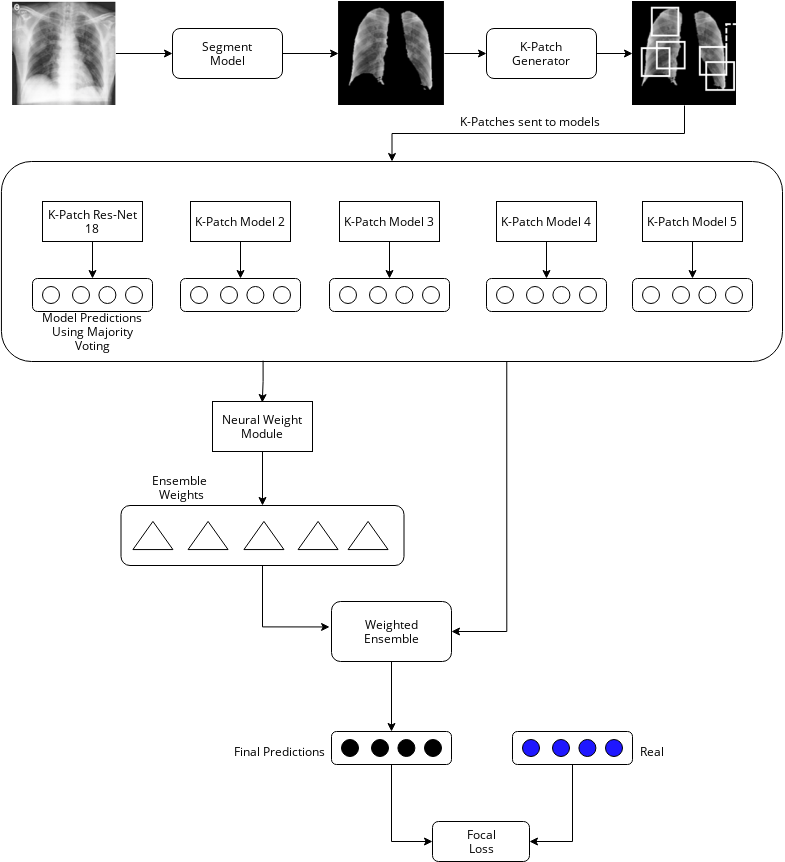
\includegraphics[width=8cm]{../doc/images/FLANNEL-IMPROVED.png}
    \caption{FLANNEL Improvement}
    \label{fig:improve}
\end{figure}

\subsection{Performance Analysis}
We will record the classification accuracy for 4 classes using F1-score. We
compare the F1-score accuracy for COVID-19 vs other classes for five base
learners, FLANNEL with ensemble strategies voting and stacking, FLANNEL with
cross entropy loss, FLANNEL with re-sampling and FLANNEL with k-patch
improvement. We use receiving operating characteristic (ROC) curve and
precision-recall (PR) curve to display classification performance against
threshold. Finally we will provide visual description of FLANNEL and proposed
improvement performance using confusion matrix.

\section{Experimental Setup}
We are planning to use \href{https://github.com/qxiaobu/FLANNEL} {FLANNEL source
    code}  as our baseline and enhance on top of it. Our codebase would be
using below software/python packages as shown in Table \ref{table:package}
\begin{table}[h]
    \centering
    \caption{Software/Tools used}
    \label{table:package}
    \begin{tabular}{|l|l|} \hline
        Software/Tool & Version \\ \hline
        Python        & 3.8.5   \\ \hline
        numpy         & 1.20.2  \\ \hline
        torch         & 1.8.1   \\ \hline
        torchvision   & 0.9.1   \\ \hline
        matplotlib    & 3.4.0   \\ \hline
        scikit-learn  & 0.24.1  \\ \hline
        pandas        & 1.2.3   \\
        \hline\end{tabular}
\end{table}

As FLANNEL model requires significant compute and GPU
resources (3 NVIDIA Tesla P100 GPUs). We would be utilizing AWS EC2 service with
instance type p3.8xlarge which provides 4 NVIDIA Tesla V100 GPUs along with 32
core CPU and 64GB RAM.

For data analysis and exploration, we are going to use Google Colab.


\begin{figure}[h]
    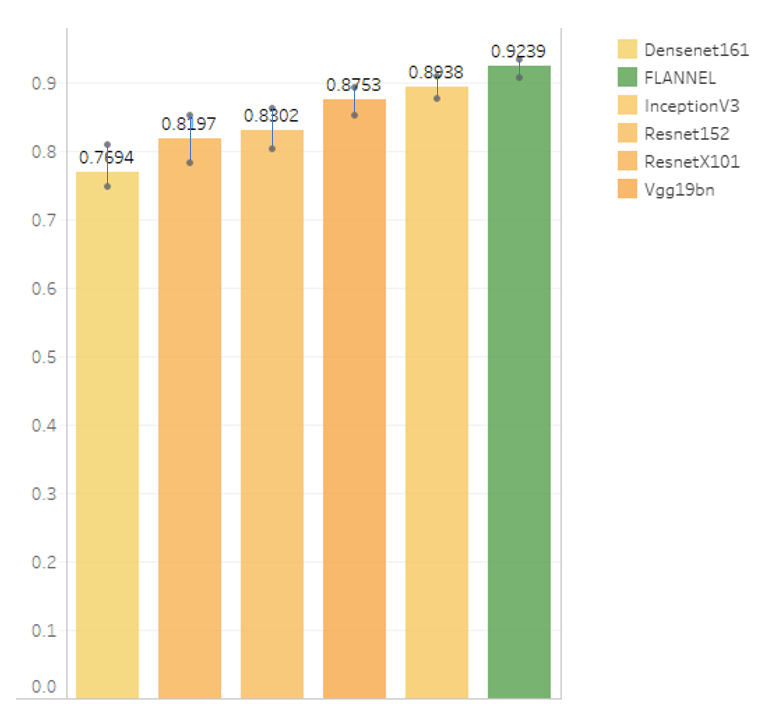
\includegraphics[width=8cm]{../doc/images/F1Score_vs_rest.png}
    \caption{FLANNEL Improvement}
    \label{fig:f1score}
\end{figure}


\newpage
%
% The following two commands are all you need in the
% initial runs of your .tex file to
% produce the bibliography for the citations in your paper.
\bibliographystyle{abbrv}
\bibliography{covid19}  % sigproc.bib is the name of the Bibliography in this case

\end{document}
